\documentclass[12pt,a4paper]{article}
\usepackage{styles}

\lstset{style=sharpc, tabsize=1}


\author{Alexander van Schie \& Oli Dias}
\title{Gruppenarbeit 1 - Cloud Fundamentals beim Provider}
\begin{document}
\maketitle
\newpage
\tableofcontents
\newpage
\section{Hands-On: Hello (Cloud) World}
%TODO Einleitung schreiben mit erklärung wieso, Start Stopp Möglichkeiten, Logfiles, Vorteil/Nachteil ggü Google App Engine
\subsection{Installationsanleitung}
Das Ziel ist es, eine Asp.Net-Core Hello-World Applikation mittels Openshift Online zu builden und deployen. Am Schluss dieser Installationsanleitung sollte dies möglich sein.


Für das Einrichten von Openshift Online müssen grob folgende Schritte durchgeführt werden:
\begin{itemize}
	\item Account und Projekt auf der Plattform erstellen
	\item GitHub Repository der Asp.Net-Core Applikation mit Openshift Projekt verbinden
	\item Applikation auf Openshift builden
	\item Applikation auf Openshift deployen
\end{itemize}
\subsubsection{Openshift Account erstellen}
Zuerst muss ein Account auf  \url{https://manage.openshift.com/sign_in} erstellt werden. Danach kann zwischen den in Abbildung \ref{fig:openshift-plan} vorgeschlagenen Plänen ausgewählt werden. Wir benutzen den Openshift Online Starter Plan.
\begin{figure}[h]
	\centering
	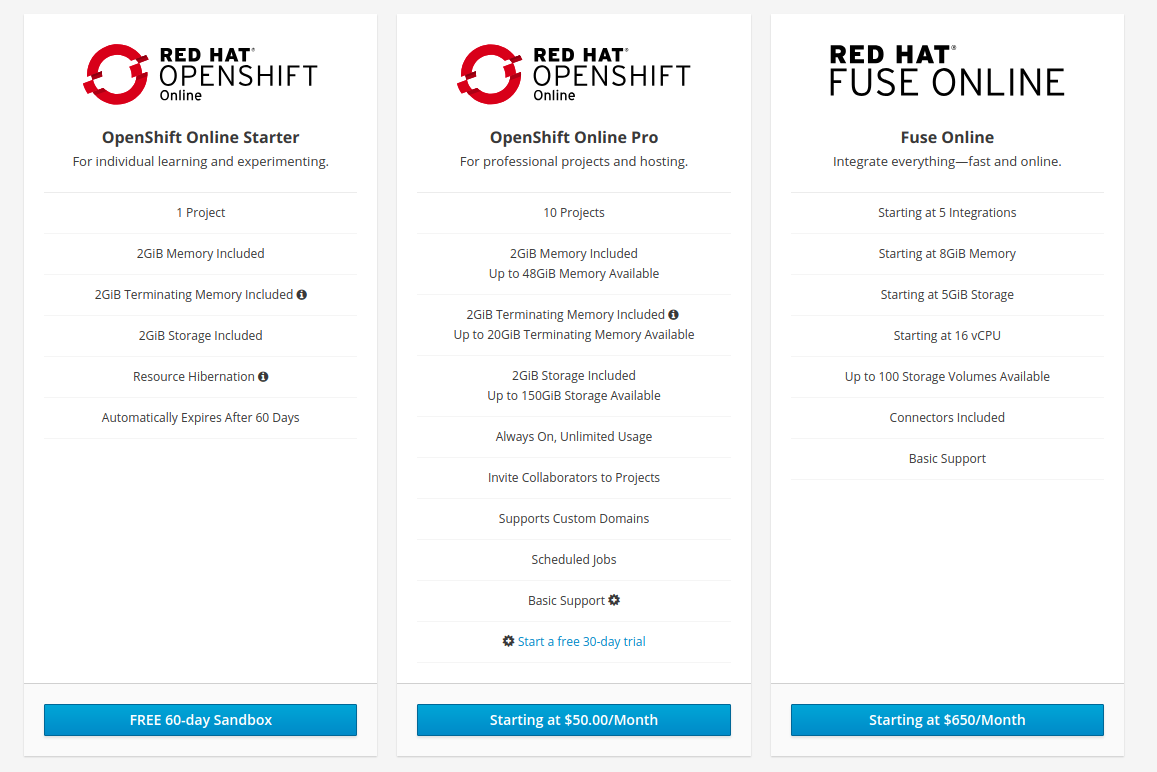
\includegraphics[width=0.7\linewidth]{img/openshift-plan}
	\caption{Gewählter Plan Openshift}
	\label{fig:openshift-plan}
\end{figure}

Dass der Account verifiziert werden kann, muss eine Telefonnummer hinterlegt werden, auf welche darauffolgend einen Bestätigungscode zugeschickt wird. 
\begin{figure}[h]
	\centering
	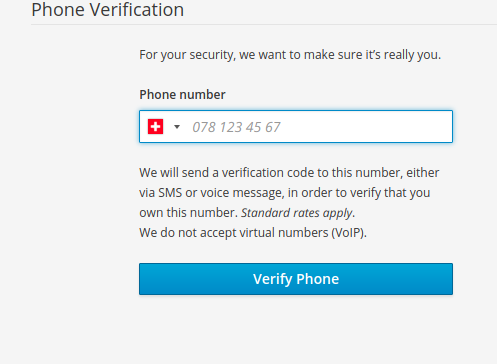
\includegraphics[width=0.7\linewidth]{img/os-phone-validation}
	\caption{Telefon Verifikation}
	\label{fig:os-phone-validation}
\end{figure}
Wurde diese eingegeben und verifiziert, erscheint eine Übersicht über das bestellte Produkt wie in Abbildung \ref{fig:os-overview} angezeigt. Daraufhin kann die Subscription bestätigt werden.
\begin{figure}[h]
	\centering
	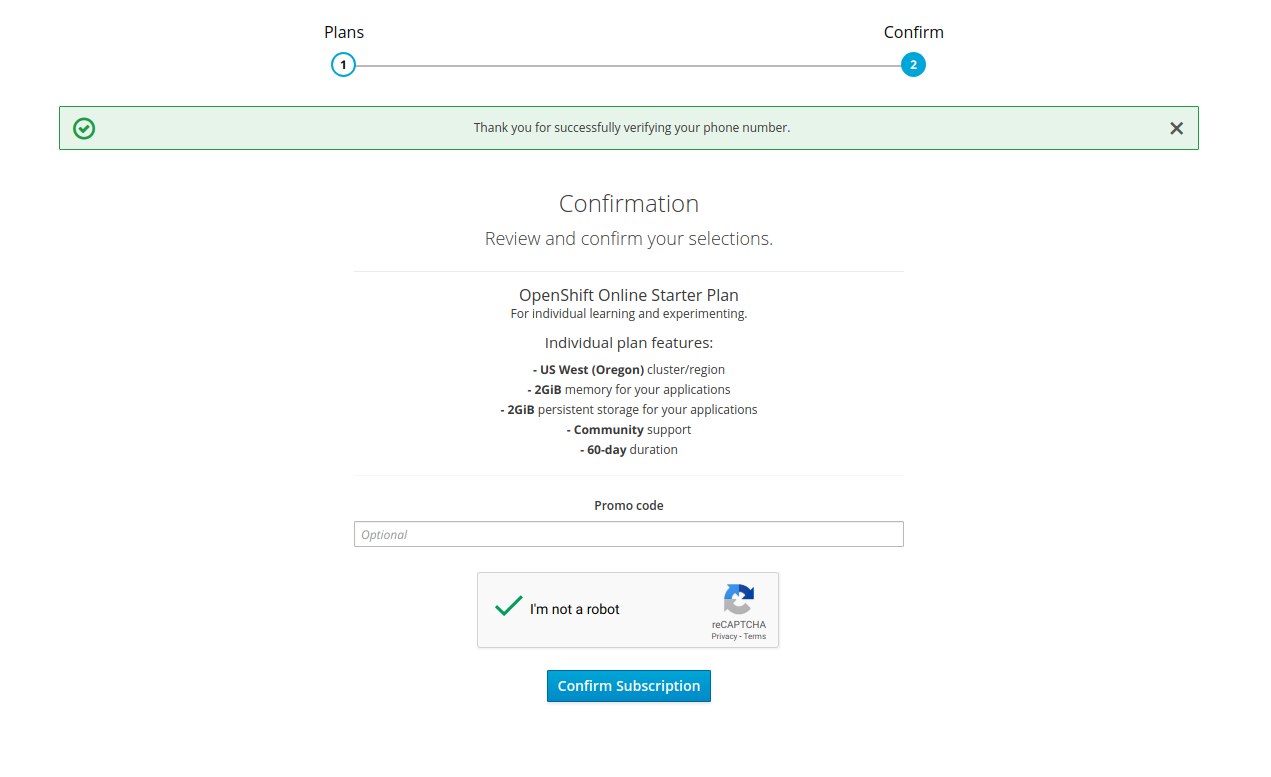
\includegraphics[width=0.9\linewidth]{img/os-overview}
	\caption{Übersicht des abgeschlossenen Plans}
	\label{fig:os-overview}
\end{figure}
Kurz nach dem Bestätigen sollte ein Bestätigungsmail eintreffen. Nach dem Bestätigen dieser kann bereits die Web Console geöffnet werden. Es wird ein Katalog mit allen Produkten von Openshift Online dargestellt (Abbildung \ref{fig:os-overview-catalog}).

\begin{figure}[h]
	\centering
	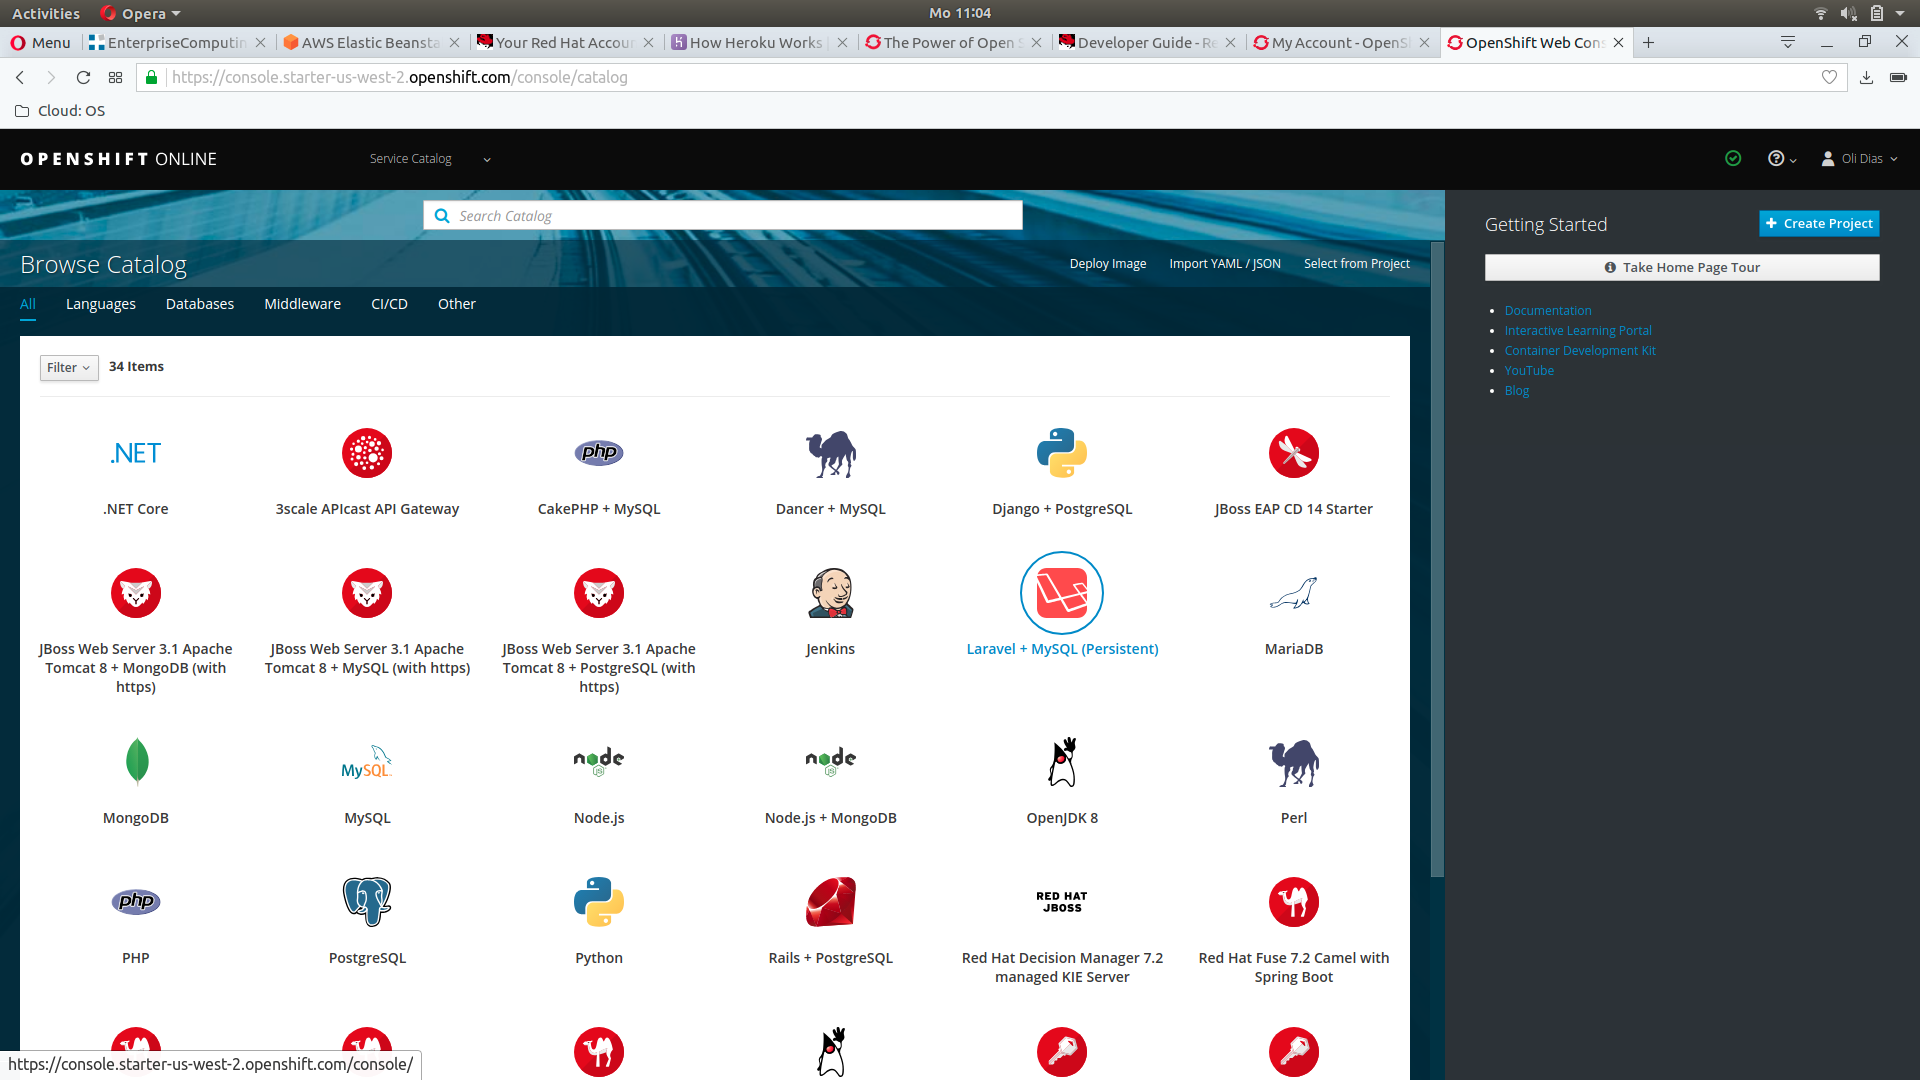
\includegraphics[width=0.7\linewidth]{img/os-overview-catalog}
	\caption{Katalog von Openshift}
	\label{fig:os-overview-catalog}
\end{figure}
Das Erstellen des Openshift Accounts ist somit abgeschlossen und die Plattform ist für das Builden und Deployen von Applikationen bereit. 
\subsubsection{Erstellen, Builden und Deployment der Applikation}
In der Web-Console können wir nun auf .NET Core Projekt clicken. Daraufhin erscheint ein Wizard, dem wir Schritt für Schritt folgen können. Falls das GitHub-Repository schon während dem Wizard hinzugefügt werden soll, muss es bereits existieren und sichtbar sein. 

Entsprechende Felder müssen gemäss Abbildung \ref{fig:os-new-config} ausgefüllt sein. Vorsicht ist bei der .NET Version geboten; wir verwenden die Version 2.2 von .NET Core. 
\begin{figure}[h]
	\centering
	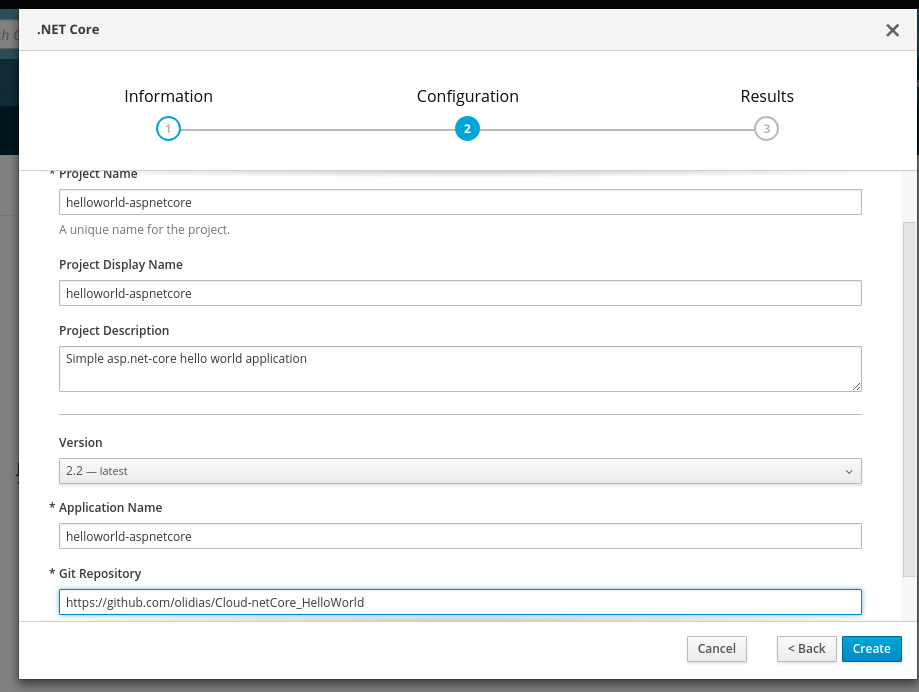
\includegraphics[width=0.7\linewidth]{img/os-new-config}
	\caption{Konfiguration des neuen Projektes}
	\label{fig:os-new-config}
\end{figure}

Sobald das Projekt in Openshift erstellt wurde, startet der Build. 
\begin{figure}[h]
	\centering
	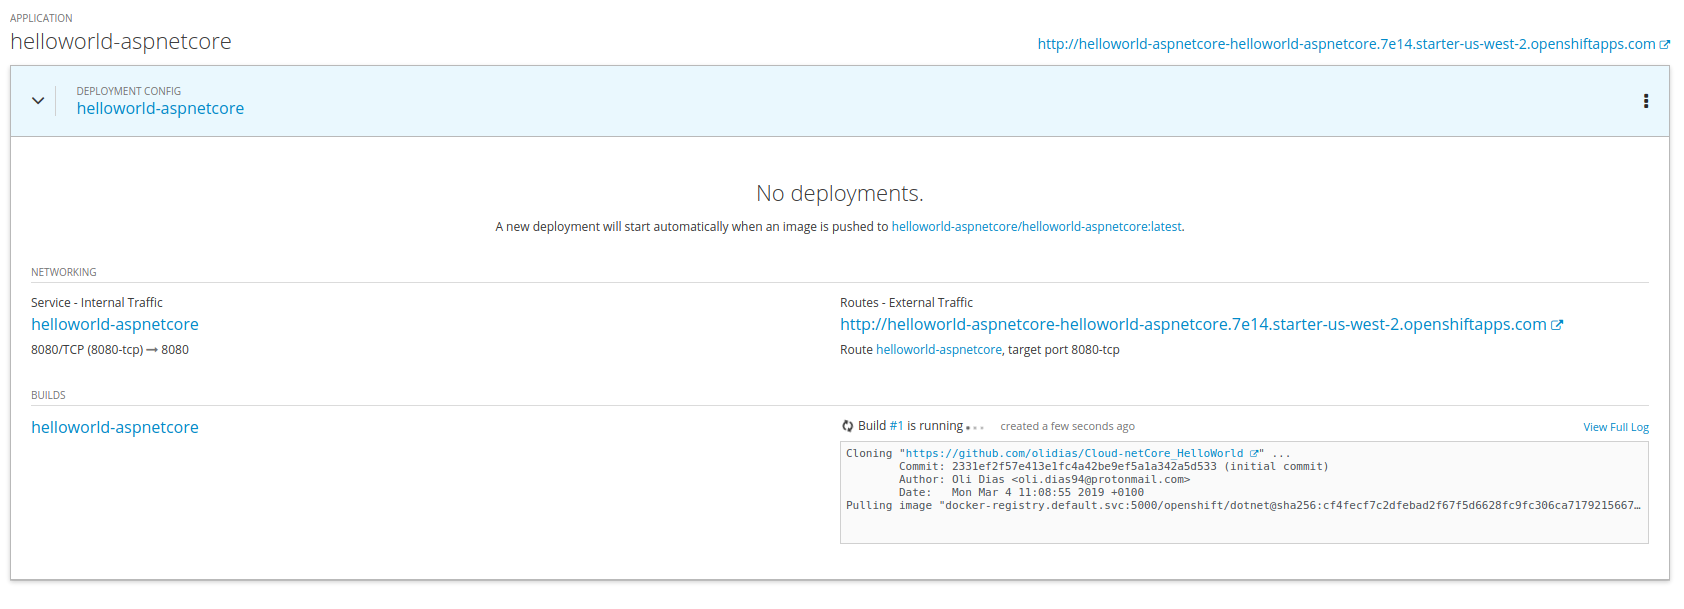
\includegraphics[width=0.7\linewidth]{img/os-building}
	\caption{Builden der .net core Applikation}
	\label{fig:os-building}
\end{figure}
Womöglich schlägt der Build aufgrund von fehlender \texttt{.s2i}-Konfiguration (Source-2-Image) fehl. Um diesen Fehler zu beheben, muss Openshift gesagt werden, wo das Startup-Projekt liegt. Dazu muss ein Ordner und File mit dem Namen \texttt{.s2i/environment} erstellt werden. Dies beinhaltet folgendes:
\begin{lstlisting}[breaklines=true]
DOTNET_STARTUP_PROJECT=HelloWorld-netcore/HelloWorld-netcore.csproj
\end{lstlisting}
Wichtig ist weiter zu beachten, dass die .net Versionen (dotnet sowie NuGet-Pakete) mit denjenigen von Openshift Cloud kompatibel sind. 

War der Build erfolgreich, muss noch das Deployment konfiguriert werden. Dazu kommt ein weiteres File mit dem Namen \texttt{run} ins \texttt{.s2i} Verzeichnis. Darin muss die Applikation noch gestartet werden. Dies funktioniert so:
\begin{lstlisting}
exec dotnet run
\end{lstlisting}
Ist auch dieser Schritt vollbracht, kann im Control Panel des Projektes zu Deployments $\rightarrow$ Routes navigiert werden. Dort erscheint eine Tabelle, wo der Hostname bereits angegeben ist und womit nun die Asp.Net-Core Applikation vom Internet her erreichbar ist.
\section{Analyse: OSSM-Definition}

\section{Konzept: Cloud Computing Patterns}

\section{Hands-On: Self Information}

\section{Analyse: Preisrecherche}

\section{Analyse: Preisvergleich eigenes Hosting, IaaS und PaaS}

\end{document}